\section{Introduction} \label{sec:introduction}
    \IEEEPARstart{F}{or} \gls{MC} \glss{MM} could be considered as an addition to a standard spatially regularised \gls{MC} technique which, not only affords a degree of temporal or gate-wise regularisation, but also allows for the interpolation of \glss{DVF} not used to fit the model (as long as a relevant \gls{SS} exists~\cite{McClelland2013}). \glss{MM} have seen attention particularly in \gls{CT}~\cite{Li2007EnhancedModel} but also \gls{MR}~\cite{Manke2002RespiratoryModels, Manber2016JointCorrection.}, however they have not yet seen a large amount of attention in clinical \gls{PET}/\gls{CT}.
    
    In previous work, the possibility of incorporating \glss{MM} in a \gls{MC} framework for \gls{NAC} \gls{TOF} \gls{PET}, where the reference position was set to the position of a breath hold \gls{Mu-Map} was investigated. This method could be used to deform both the gates to the reference position as well as the reference position to the gates. It was found that the combination of both the \gls{MM} and \gls{TOF} was sufficient to perform an \gls{AC} reconstruction with \gls{MC}, without introducing artefacts, while increasing resolution and quantification accuracy~\cite{Whitehead2019ImpactPET, Whitehead2020PET/CTFields, Whitehead2021ComparisonMap}. This work seeks to extend the method further by incorporating \gls{MLACF} as an initialisation technique, which provides volumes with greater contrast without introducing bias~\cite{Mizuta2022InitialPET}. Secondly, low bin count pseudo-phase gated data is used for the \gls{MM} fitting while high count displacement gated data is used for the output, exploiting the \glss{MM} ability to interpolate \glss{DVF} to significantly reduce computation time. Thirdly, a diffeomorphic velocity field parameterised registration method was used which provided \glss{DVF} free from folding, thus being able to be inverted. Furthermore, this work uses more realistic simulation and count levels from existing clinical scanners, compared to previous work (where more simple registration methods would fail).
    
    A method incorporating \glss{MM} for dynamic \gls{PET}/\gls{CT}, was proposed and tested on clinical data in~\cite{Chan2018Non-RigidPET}. Additionally, a method incorporating \gls{MLACF} for \gls{PET}/\gls{CT}, was proposed in~\cite{Lu2018RespiratoryData}. The work presented here, differentiates itself not only by the ways mentioned above but also by using a \gls{2D} \gls{SS}, rather than a \gls{1D} \gls{SS}, thus both inter- and intra-gate motion can be included in the model, at the expense that each gate contains fewer counts. Additionally, the group-wise method, presented here, makes use of an iterative \gls{MC} algorithm rather than using only a pair-wise method.

% \vspace{-0.3cm}

\section{Methods} \label{sec:methods}
    \subsection{XCAT Volume Generation} \label{sec:xcat_volume_generation}
        \gls{XCAT}~\cite{Segars2010} was used to generate $480$ volumes over a \SI{240}{\second} period using a respiratory trace, derived from \gls{MR} navigator patient data. The max displacement of \gls{AP} and \gls{SI} motion, was set to \SI{1.2}{\centi\metre} and \SI{2.0}{\centi\metre} respectively. Activity concentrations were derived from a static \gls{18F-FDG} patient scan. The \gls{FOV} included the base of the lungs, diaphragm and the top of the liver with a \SI{20}{\milli\metre} diameter spherical lesion (smaller than the max displacement, due to \gls{RM}) was placed into the base of the right lung (within the max displacement, due to \gls{RM}, of the diaphragm).
    
    % \vspace{-0.3cm}
    
    \subsection{PET Acquisition Simulation} \label{sec:pet_acquisition_simulation}
        \gls{PET} acquisitions were simulated (and reconstructed) using \gls{STIR}~\cite{Thielemans2012, Nikos2019} through \gls{SIRF}~\cite{Ovtchinnikov2017}, to forward project data using the geometry of a \gls{GE} Discovery $710$. Attenuation was included using the relevant \glss{Mu-Map} generated by \gls{XCAT}. Pseudo-randoms and scatter were added. Randoms were added by summing a scaled uniform forward projection to the simulation sinogram. Pseudo-scatter was added by summing a scaled and smoothed forward projection of the activity data at each time point to the simulation sinogram. The smoothing parameter was optimised to give scatter with a similar distribution to a GATE gate simulation. A full scatter simulation was not performed due to software limitations.
        
        Noise was simulated, such that data matched an acquisition over \SI{240}{\second}, emulating a standard single bed position acquisition. The count rate was selected to match that of research scans, i.e. below that of diagnostic clinical scans. This count rate was selected as a 'worst case scenario'.
        
        A respiratory \gls{SS} was generated using \gls{PCA}~\cite{Thielemans2011}. The magnitude of this signal and its gradient, was used to initially gate data into four respiratory bins using pseudo-phase gating. This gating scheme gave a bin centred on the maximum and minimum amplitude and gradient of the \gls{SS}. This is useful as it gives the minimum reasonable number of gates to fit a \gls{2D} \gls{MM} (a plane). For the purpose of the \gls{MM} fitting, \gls{SS} values were determined for the post-gated data by taking an average of the \gls{SS} values of data in each bin.
        
    \subsection{MLACF Image Reconstruction} \label{sec:mlacf_image_reconstruction}
        Data were reconstructed using \gls{MLACF} with seven full iterations and $24$ subsets for the activity update and iterating until convergence for the attenuation update (where an attenuation update is performed before every activity iteration)~\cite{Mizuta2022InitialPET}. \gls{MLACF} was initialised using one iteration of \gls{MLEM} where the breath hold \gls{CT} was used for \gls{AC} (the \gls{ACF} were still initialised with all ones), this gave a small improvement to results without introducing bias. Between iterations the activity volume and \gls{ACF} volume were normalised and had a small value added to them, this was to aid with stabilising the reconstruction, with \gls{MLACF} the scale of the reconstruction is arbitrary. A quadratic prior was included to promote smoothness of the \gls{ACF} volume.
    
    % \vspace{-0.3cm}
    
    \subsection{Registration} \label{sec:registration}
        Before being registered, each volume underwent pre-processing. Including replication of end-slices, smoothing and standardisation. This pre-processing was only applied to intermediate data and was not used for the final output of the method.
        
        Group-wise registration was used, where after an initial pair-wise registration step a new reference volume was resampled. Registration to the new reference volume, followed by another resample, continued for a set number of iterations. NiftyReg~\cite{Modat2010} was used to perform registrations using a diffeomorphic velocity field B-spline parameterisation. \gls{CPG} spacing of the B-spline coefficients, \gls{BE} regularisation term weight and number of iterations were tuned using a grid search.
    
    % \vspace{-0.3cm}
    
    \subsection{Motion Model Estimation} \label{sec:motion_model_estimation}
        \glss{MM} were fit as a direct \gls{RCM} on the \glss{CPG} from~\Fref{sec:registration} and the \gls{SS} from~\Fref{sec:pet_acquisition_simulation}. A weighted \gls{LR} was used, where the weighting was taken based on the number of counts in each gate. Once a \gls{MM} was fit, new \glss{DVF} were generated for each gate, using the \gls{SS} values used to fit the \gls{MM}. \gls{MM} fitting occurred between iterations, the \glss{DVF} generated by the \gls{MM} were used to resample the new target volume at each iteration.
        
        Between each iteration the resampled volume was registered to the position of the \gls{Mu-Map}. The \glss{CPG} for both the group-wise registration and this registration were then composed together before a \gls{MM} was fit on them. With the diffeomorphic nature of the registration this would give a \gls{MM} which could generate \glss{DVF} to and from the gates to the \gls{Mu-Map}.
    
    % \vspace{-0.3cm}
    
    \subsection{Motion Corrected Image Reconstruction with AC} \label{sec:motion_corrected_image_reconstruction_with_ac}
        Data were re-gated using the magnitude of \gls{SS} and its gradient, to gate data into $30$ respiratory bins using displacement gating ($10$ amplitude and $3$ gradient bins).
        
        Data were re-reconstructed with \gls{AC}, deforming the \glss{Mu-Map} using the inverse of the \glss{DVF} from~\Fref{sec:motion_model_estimation} using \gls{OSEM} with two full iterations and $24$ subsets (parameters are equivalent to standard clinical practise)~\cite{Hudson1994}. \gls{MC} was then applied using \glss{DVF} from~\Fref{sec:motion_model_estimation}. Volumes were post-filtered using a Gaussian smoothing, with a \gls{FWHM} of \SI{6.4}{\milli\metre} in the transverse plane (equivalent to three voxels) and a normal Z filter, this is equivalent to standard clinical practise.
    
    % \vspace{-0.3cm}
    
    \subsection{Evaluation} \label{sec:evaluation}
        In addition to the reconstructions performed in~\Fref{sec:motion_corrected_image_reconstruction_with_ac}, data were also \gls{MC} in the same was as in~\Fref{sec:registration} and~\Fref{sec:motion_model_estimation} but without using the low bin count pseudo-phase gated data initialisation. Furthermore data were reconstructed without \gls{MC}, using either a sum of all \glss{Mu-Map} (to emulate an \gls{AV-CCT}), or the end inhalation \gls{Mu-Map}. For the present evaluation, the volumes without \gls{MC} were registered to the position of the end inhalation \gls{Mu-Map}. Additionally, \glss{DVF} generated by each method were also applied to noiseless data for visual analysis.
        
        Comparisons used included: \gls{COM} of a volume containing only the lesion over time, a profile over the lesion, \gls{SUV}\textsubscript{max} and \gls{SUV}\textsubscript{peak} (defined following \gls{EANM} guidelines~\cite{Boellaard2015FDG2.0}).

% \vspace{-0.3cm}

\section{Results} \label{sec:results}
    \begin{figure*}
        % \vspace{-0.3cm}
        
        \centering
        
        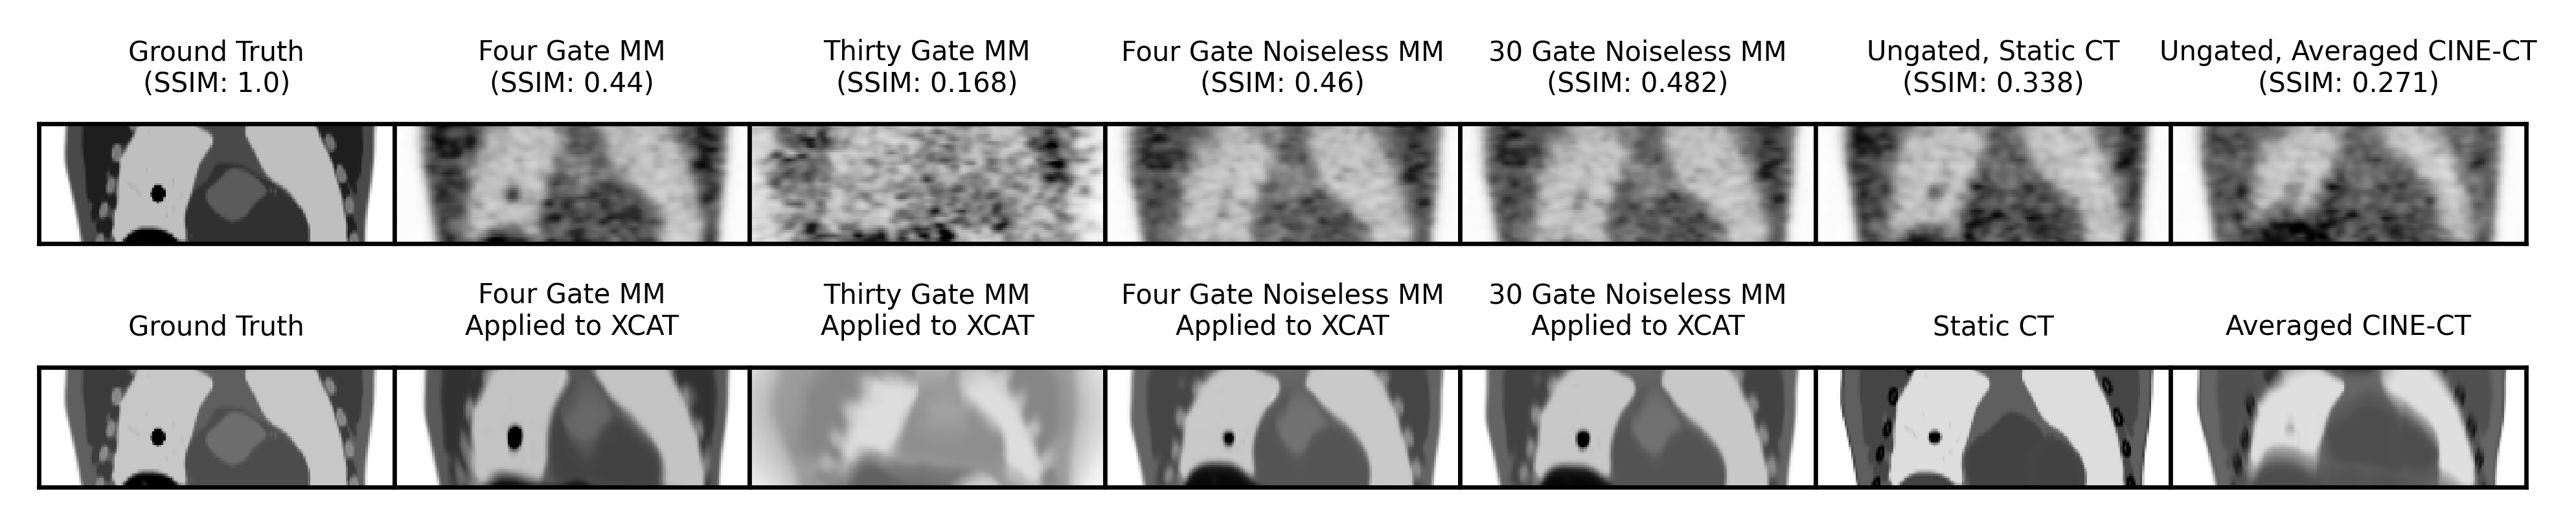
\includegraphics[width=1.0\linewidth]{figures/visual_analysis.png}
        
        % \vspace{-0.3cm}
        
        \captionsetup{singlelinecheck=false, justification=centering}
        \caption{First row contains \gls{AC} \gls{MC} reconstructions and the second row contains the result of applying the final \gls{MM} on the original \gls{XCAT} volumes for; ground truth, low gate resolution \gls{MM}, high gate resolution \gls{MM}, low gate resolution \gls{MM} noiseless, high gate resolution \gls{MM} noiseless, \gls{NMC} breath hold \gls{CT}, \gls{NMC} \gls{AV-CCT}. Colour map ranges are consistent for all images in each row.}
        
        \label{fig:visual_analysis}
        
        % \vspace{-0.3cm}
    \end{figure*}
    
    \begin{figure}
        % \vspace{-0.3cm}
        
        \centering
        
        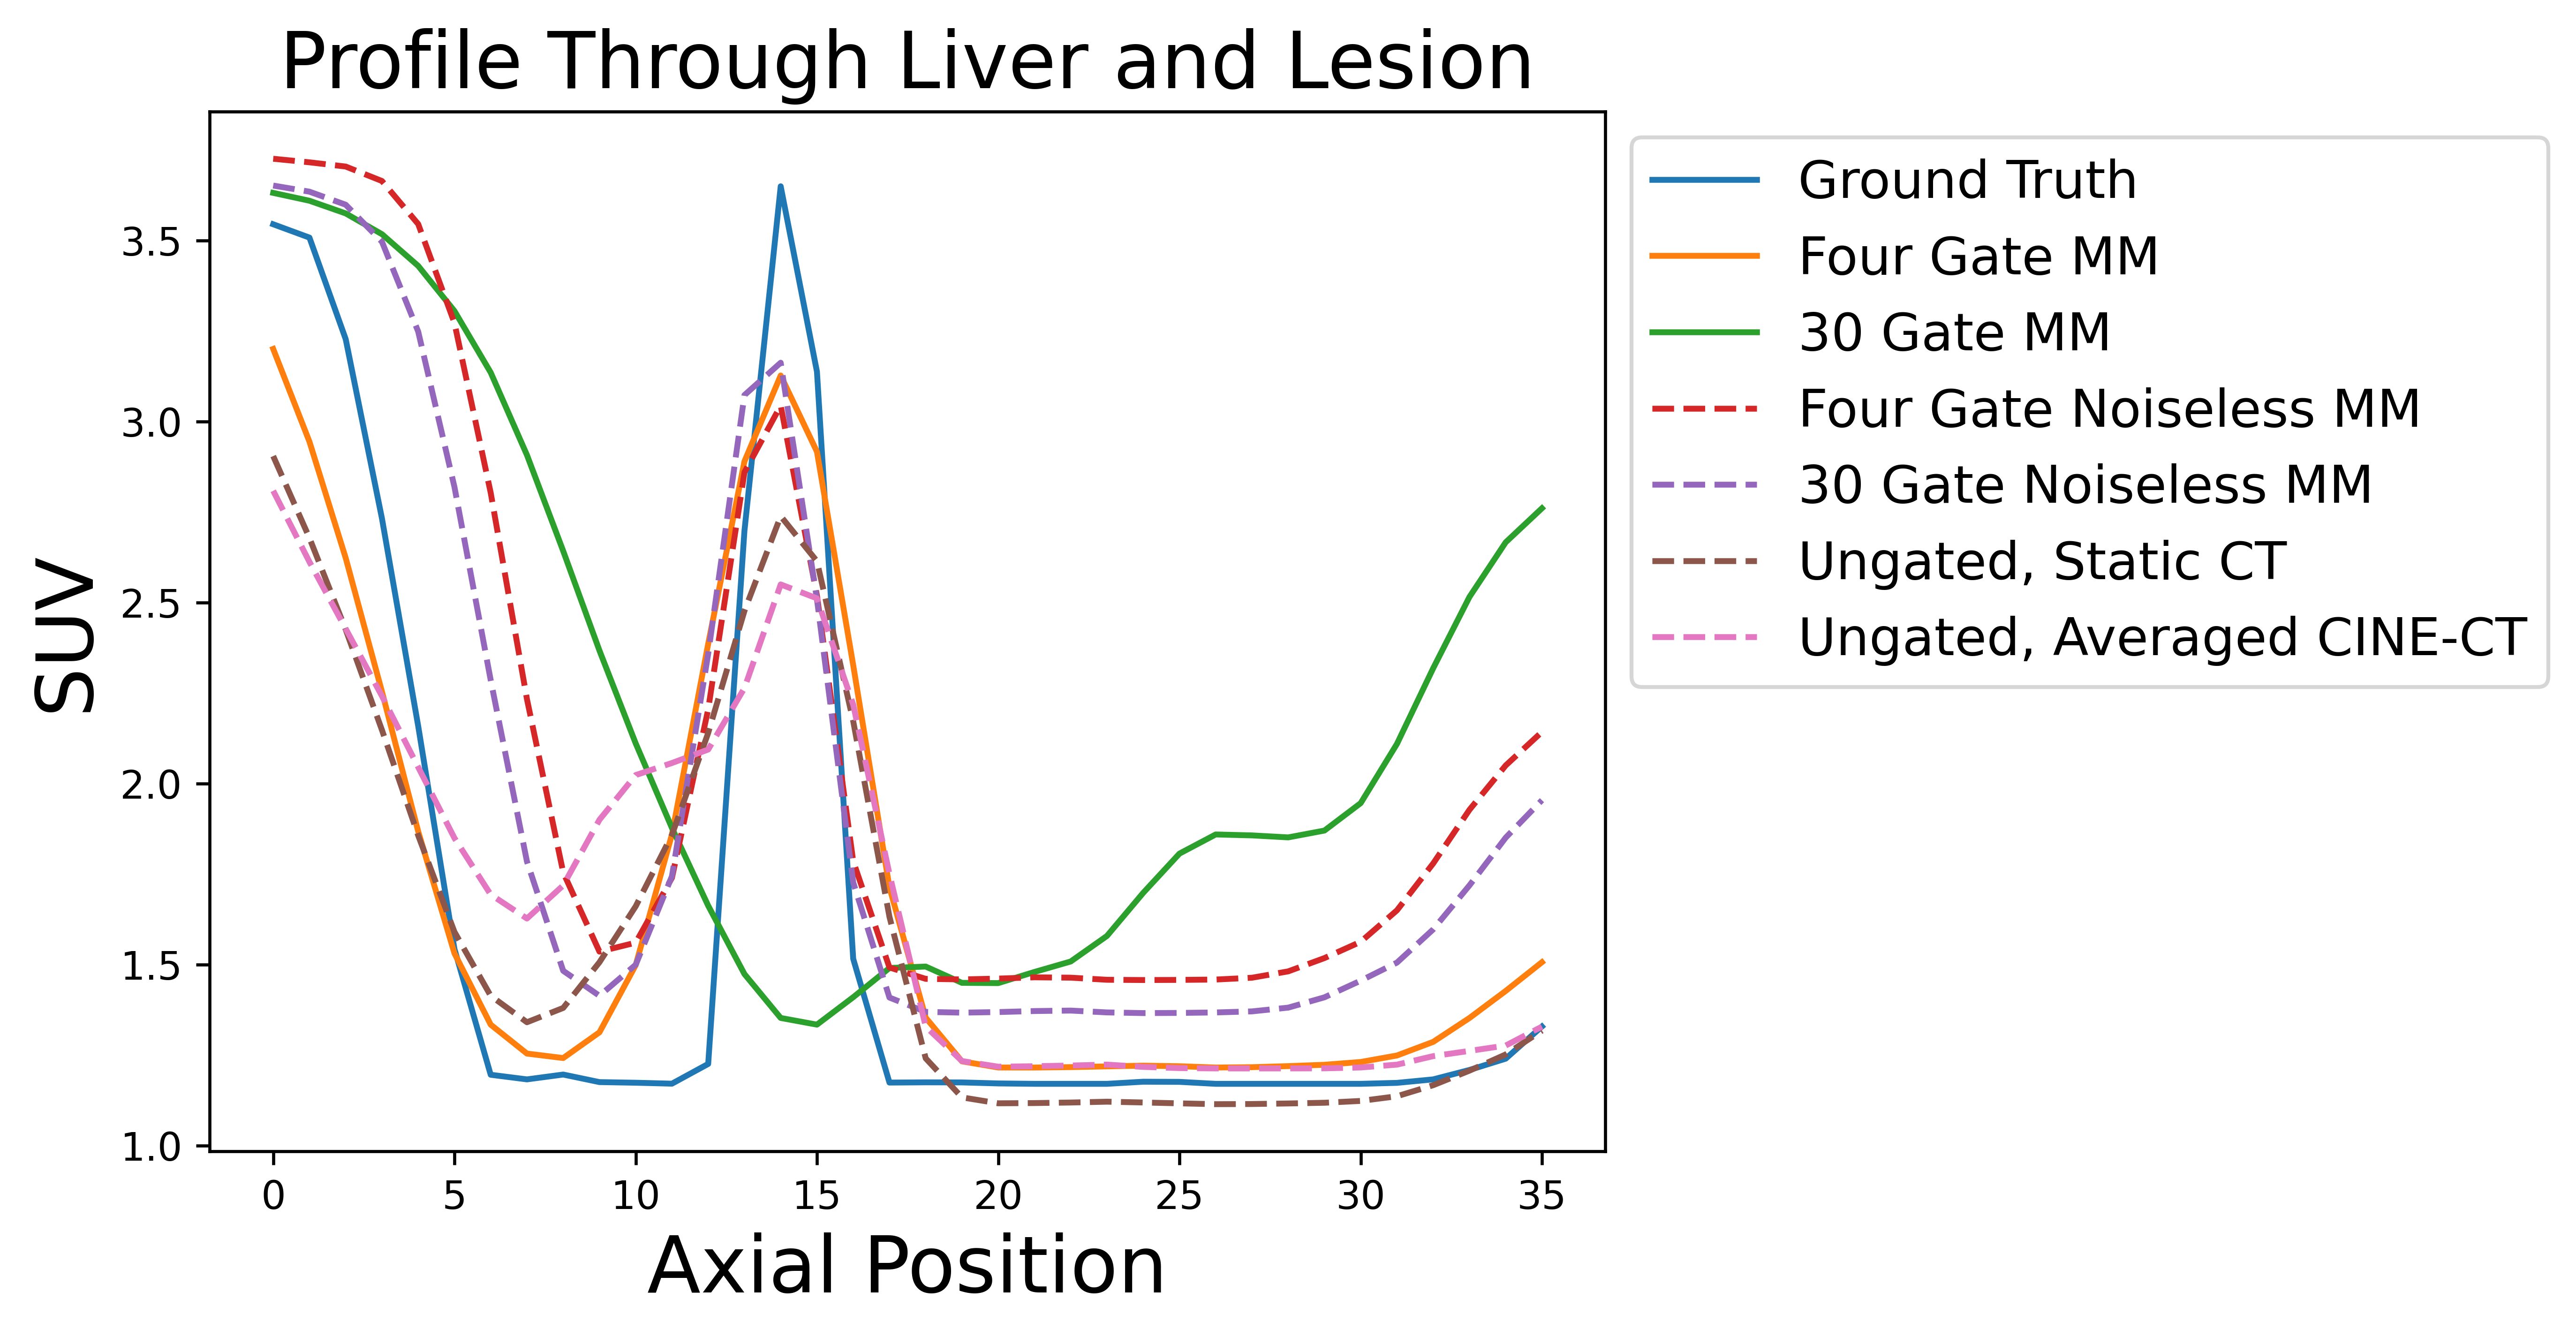
\includegraphics[width=1.0\linewidth]{figures/profile.png}
        
        % \vspace{-0.3cm}
        
        \captionsetup{singlelinecheck=false, justification=centering}
        \caption{A profile across the lesion for; ground truth, low gate resolution \gls{MM}, high gate resolution \gls{MM}, low gate resolution \gls{MM} noiseless, high gate resolution \gls{MM} noiseless, \gls{NMC} breath hold \gls{CT}, \gls{NMC} \gls{AV-CCT}.}
        
        \label{fig:profile}
        
        % \vspace{-0.3cm}
    \end{figure}
    
    \begin{table}
        \centering
        
        \captionsetup{singlelinecheck=false, justification=centering}
        \caption{Comparison of \gls{SUV}\textsubscript{max} and \gls{SUV}\textsubscript{peak} for; ground truth, low gate resolution \gls{MM}, high gate resolution \gls{MM}, low gate resolution \gls{MM} noiseless, high gate resolution \gls{MM} noiseless, \gls{NMC} breath hold \gls{CT}, \gls{NMC} \gls{AV-CCT}.}
        
        \resizebox*{1.0\linewidth}{!}
        {
            \begin{tabular}{||c|cc||}
                \hline
                \textbf{\gls{SUV}}                                  & \textbf{Max}  & \textbf{Peak} \\
                \hline
                \textbf{Ground Truth}                               & $8.61$        & $7.82$ \\
                \hline
                \textbf{Low Gate Resolution \gls{MM}}               & $7.90$        & $6.08$ \\
                \textbf{High Gate Resolution \gls{MM}}              & $1.74$        & $1.30$ \\
                \hline
                \textbf{Low Gate Resolution \gls{MM} Noiseless}     & $7.91$        & $6.10$ \\
                \textbf{High Gate Resolution \gls{MM} Noiseless}    & $7.82$        & $5.99$ \\
                \hline
                \textbf{\gls{NMC} Breath Hold \gls{CT}}             & $6.46$        & $4.95$ \\
                \textbf{\gls{NMC} \gls{AV-CCT}}                     & $5.56$        & $4.37$ \\
                \hline
            \end{tabular}
        }
        \label{tab:suv}
        
        % \vspace{-0.3cm}
    \end{table}
    
    A visual comparison of the reconstructed images (see ~\Fref{fig:visual_analysis}) shows that the high gate resolution \gls{MM} method performs quite poorly, most probably due to the high level of noise apparent in the volumes. Conversely, the low gate resolution \gls{MM} method appears to be able to \gls{MC} the data without being too adversely affected by the noise levels.
     
    The peak of the profile (see~\Fref{fig:profile}) is comparable where noise is included and where it is not included for the low gate resolution \gls{MM} method. However, there does not seem to be a peak for the high gate resolution \gls{MM} method. The peak is greater for the \gls{MC} methods than where it is not included.
     
    \gls{SUV} results show that unnecessarily increasing the number of gates for the \gls{MM} reduces \gls{SUV} when high levels of noise are apparent in the data (see~\Fref{tab:suv}).

% \vspace{-0.3cm}

\section{Discussion and Conclusions} \label{sec:discussion_and_conclusions}
    Results from a visual analysis, a comparison of profiles and \gls{SUV}, show that using a low number of gates for \gls{MM} fitting, not only does not negatively impact results, but in fact can improve them when there is a high level of noise apparent in the gates. In addition to this the execution time from using a reduced number of gates is significantly reduced.
    
    In the future, work will focus on initially evaluating the method on patient data, before moving on to rather than fitting the \gls{MM} as a post-processing step fitting it incrementally with reconstruction.
    